\documentclass[10pt,a4paper]{llncs}
\usepackage[utf8]{inputenc}
\usepackage[english]{babel}
\usepackage{amsmath}
\usepackage{amsfonts}
\usepackage{amssymb}
\usepackage{makeidx}
\usepackage{mathdots}
\usepackage{graphicx}
\usepackage{ textcomp }
\usepackage{subcaption}
\usepackage{caption}
\usepackage{fancybox}
\usepackage{multicol}
\usepackage{multirow,array}
%\usepackage{geometry}
\pagestyle{plain}
\renewcommand{\labelitemi}{$\bullet$}
\DeclareMathOperator*{\argmin}{arg\, min}
\usepackage{vmargin}

%\setpapersize{A4}
%\setmargins{2cm}% margen izquierdo
%{1.5cm}% margen superior
%{17cm}% anchura del texto
%{23.6cm}% altura del texto
%{10pt} % altura de los encabezados
%{1cm}% espacio entre el texto y los encabezados
%{0pt}% altura del pie de página
%{2cm}% espacio entre el texto y el pie de página
\usepackage{hyperref}
\title{Image inpainting and completion}
\author{Onofre Martorell Nadal\\onofremartorelln@gmail.com}

\institute{Universitat Oberta de Catalunya}
\begin{document}
\maketitle
\thispagestyle{plain}
\begin{abstract}
This document is a brief explanation of the work done the project of the Module 2 of the master of Computer Vision. The goal of the project was to implement an algorithm of image completion based on different variational and graphical models. The document is structured as follows: first, a short introduction of the problem; later, the steps done so as to solve the problem and at the end, an example of the solution obtained and the conclusions.
\end{abstract}
\keywords{image completion, image inpainting, image segmentation, image editing}
\section{Introduction}
Every once in a while, we all wish we could erase something from
our old photographs. A garbage truck right in the middle of a
charming Italian piazza, an ex-boyfriend in a family photo,...
Other times, there is simply missing data in some areas of the image.
An aged corner of an old photograph, a dead bug on the camera lens or the red parts of the image \ref{img:goal_image}. The way to restore those images is through a technique called image completion.
\noindent
Image completion (also called hole-filling) is the task
of filling in or replacing an image region with new image data such
that the modification can not be detected. This does not mean that we can recover the information that it was originally there, it means that we can add new information in order that a human eye can not detect that this process has been done in the image.

\noindent
With that, the aim of this project is to present an algorithm for image completion based on different techniques based on variational and graphical models. In order to have a more clear structure, the document has been divided in four parts: inpainting, segmentation, Poisson editing and completion, which corresponds with sections \ref{sec:inpaint} to \ref{sec:segmentation}. Each section contains a brief explanation of the technique used in an step and the way to implement it. After all that, the results are presented using image \ref{img:goal_image} as an example of the process. 
\begin{figure}[b]
\begin{center}
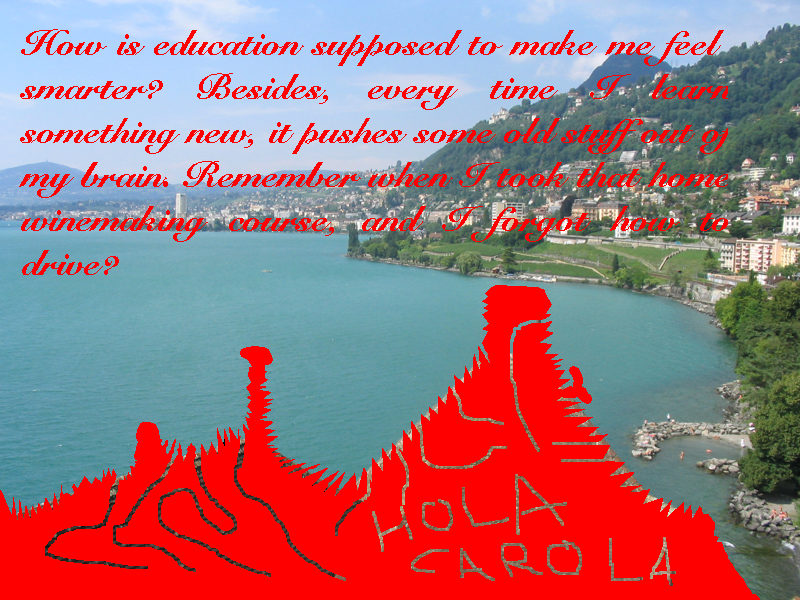
\includegraphics[scale=0.6]{Goal_image}
\caption{example image in which we will perform the image completion algorithm.}
\label{img:goal_image}
\end{center}
\end{figure}
\section{Image inpainting}\label{sec:inpaint}
\subsection{Formulation of the model}
The first step done is image inpainting, which consists on reconstructing lost parts of the image. Concretely, we will use this technique in order to eliminate the letters from our image. The way to do it is the following: let $f:\Omega\rightarrow\mathbb{R}$ be a given grayscale image and let $D\subset\Omega$ be an open set representing the region to be inpainted. With this, the inpainted image $u$ can be find as the solution of the functional
\begin{equation}
\begin{cases}
\displaystyle\argmin\limits_{u\in W^{1,2}(\Omega)}\int _D |\nabla u(x)|^2dx,\\
u|_{\partial D} = f
\end{cases}
\label{eq:inpaint_funcional}
\end{equation}
The interpretation of this functional is that we want to find the image $u$ in which the change of color between neighbour pixels is small and that is similar to the original image in the boundary of the set.
\subsection{Numerical implementation}
The minimum of the functional from the equation \ref{eq:inpaint_funcional} also satisfies the associated Euler-Lagrange equation
\begin{equation}
\left\lbrace
\begin{array}{l l}

u_{xx}+u_{yy} = 0& \text{in }D \\
u = f & \text{in }\partial D.

\end{array}\right.
\label{eq:inpaint_E-L}
\end{equation}
Given a pixel $(i, j)$ from the image and belonging to $D$, this equation can be discretizised as \cite{hoffman2001numerical} \cite{Note1}
\begin{equation}
\frac{1}{h_j^2}u_{i,j-1} + \frac{1}{h_i^2}u_{i-1, j} - \bigg(\frac{2}{h_i^2}+\frac{2}{h_j^2}\bigg)u_{i,j} + \frac{1}{h_i^2}u_{i+1,j} + \frac{1}{h_j^2}u_{i, j+1} = 0.
\label{eq:inpaint_aproximacio}
\end{equation}
Moreover, for the boundary of the image we add one row or column to each side of the image and we compute the Neumann boundary conditions. For example, at the east side, we get
\begin{equation}
\frac{u_{i, 1} - u_{i, 2}}{h_j} = 0\Longrightarrow u_{i,1} = u_{i, 2}.
\label{eq:inpaint_point_boundary}
\end{equation}
And for the points not belonging to $D$ we have
\begin{equation}
u_{i, j} = f_{i, j}.
\label{eq:inpaint_normal_points}
\end{equation}
To sum up, we sort the pixels of the image as
\begin{equation}
x = (u_{1,1}, u_{2,1}, \cdots, u_{i, j}, u_{i+1, j}, \cdots ,u_{n_i + 2,n_j + 2})^T
\end{equation}
and for each pixel we create its equation (\ref{eq:inpaint_aproximacio}, \ref{eq:inpaint_point_boundary} or \ref{eq:inpaint_normal_points}) corresponding with the type of pixel it is. Doing that, the inpainted image $u$ can be found as the solution of the linear system 
\begin{equation}
Ax = b,
\end{equation}
where $A$ is the matrix of coefficients and $b$ is the vector of independent terms for each equation. As one have may noticed, we defined $f$ as a grayscale image, but in fact our image is colorscale. The way to apply this algorithm to image \ref{img:goal_image} is by performing it on each channel of color (RGB). This results can also be improved using another algorithm such the one explained in \cite{bresson2008fast}.
\section{Image segmentation}\label{sec:segmentation}
Once we have eliminated the letters, the next step is to remove the other red part of the image, and the way to do it will be by copying a zone from another image that fits on our image. This step will be done on section \ref{sec:completion}, but before that we need to do some steps: as on can see in the image \ref{img:goal_image}, the boundary of the red zone of the bottom is not smooth. Because of that, the next step we will do is to make a segmentation of the image in order to have an smoother boundary. The way to segment the image will be done using a technique developed by Mumford and Shah in \cite{mumford1989optimal} and improved by Chan and Vese in \cite{chan2001active}. 
\subsection{Formulation of the model}
The Chan-Vese segmentation finds the curve $C$ that is the boundary of the segmentation. As it is difficult to manipulate $C$ we will use a function $\phi$ and the $C$ will be the zero crossing of $\varphi$ that is 
\begin{equation}
C = \{x\in \Omega:\varphi(x) = 0\}.
\end{equation}
With this the functional that we need to minimize is

\begin{equation}
\begin{split}
\text{arg min}_{c_1, c_2, \varphi}\ \mu \int_{\Omega}\delta(\varphi(x))|\nabla\varphi(x)|dx+\nu \int_{\Omega}H(\varphi(x))dx\, + \lambda_1\int_{\Omega}|f(x)-c_1|^2H(\varphi(x))dx \\+ \lambda_2\int_{\Omega}|f(x) -c_2|^2(1-H(\varphi(x)))dx,
\end{split}
\label{eq:segment_functional}
\end{equation}
where $H$ denotes the Heaviside function and $\delta$ the Dirac mass, its distributional derivative:
\begin{equation}
H = \left\lbrace\begin{array}{l l}
1&\quad t\geq 0,\\
0 &\quad  t<0
\end{array}\right. ,\quad \delta(t) = \frac{d}{dt}H(t).
\label{eq:segment_Heaviside}
\end{equation}

\noindent
Note that we cannot derive $H(t)$. Because of that, in the implementation we take the Heaviside function and the Dirac mass as
\begin{equation}
H_{\varepsilon}(t) = \frac{1}{2}\bigg(1 + \frac{2}{\pi}\arctan \bigg(\frac{t}{\varepsilon}\bigg)\bigg),\quad\delta_{\varepsilon} = \frac{\varepsilon}{\pi(\varepsilon^2)+t^2)}.
\end{equation}
\subsection{Numerical implementation}
The functional \ref{eq:segment_functional} is minimized as in \cite{getreuer2012chan} and the way to do it is the following: at each iteration we do this steps
\begin{enumerate}
\item[1.] Update $c_1$ and $c_2$ as 
\begin{equation}
c_1 = \frac{\int_{\Omega}f(x)H(\varphi(x))dx}{\int_{\Omega}H(\varphi(x))dx} \text{ and } c_2 = \frac{\int_{\Omega}f(x)(1-H(\varphi(x)))dx}{\int_{\Omega}(1-H(\varphi(x)))dx}.
\end{equation}

\item [2.] Evolve $\varphi$ using the semi-implicit Gauss-Seidel method \cite{aubert1997variational}

\begin{equation}
\begin{split}
\varphi_{i,j}^n = [\varphi_{i,j}^n + dt\cdot\delta_{\varepsilon}(\varphi_{i,j}^n)(A_{i,j}\varphi_{i+1,j}^n) + A_{i-1,j}\varphi_{i-1,j}^{n+1}+B_{i,j}\varphi_{i,j+1}^n+\\
B_{i, j-1}\varphi_{i,j-1}^{n+1}-\nu - \lambda_1(f_{i,j}-c_1)^2+\lambda_2(_{i,j}-c_2)^2) ]\\
\big/[1 + dt\cdot\delta_{\varepsilon}(\varphi_{i,j}^n)(A_{i,j} + A_{i-1,j} + B_{i,j} + B_{i,j-1})],
\end{split}
\end{equation}


where
\begin{equation}
A_{i,j} = \frac{\mu}{\sqrt{\eta^2 + (\varphi_{i+1,j}^n-\varphi_{i,j}^n)^2+((\varphi_{i,j+1}^n-\varphi_{i,j-1}^{n+1})/2)^2}}
\label{eq:segment_A}
\end{equation}
\begin{equation}
B_{i,j} = \frac{\mu}{\sqrt{\eta^2+((\varphi_{i+1,j}^n-\varphi_{i-1,j}^{n+1})/2)^2 + (\varphi_{i,j}^n-\varphi_{i+1,j}^n)^2}}
\label{eq:segment_B}
\end{equation}


\item [3.] If we have reached the maximum number of iterations or the difference $\max(|\varphi^{n+1}-\varphi|)$ is lower than a given tolerance, we stop the algorithm.
\end{enumerate}


As one can notice, the functional \ref{eq:segment_functional} has many different parameters. In order to clarify the use of each of them and the value used in the implementation, the table \ref{table:paremeters} has been created. 

\begin{table}
\begin{center}
\begin{tabular}{|c|l|c|}
\hline
Parameter & \multicolumn{1}{c|}{Use}  & \hspace{0.2cm}Value in implementation\hspace{0.2cm}\\
\hline
$\mu$ & \hspace{1pt} Weighs the length of the curve $C$&1\\
\hline
$\nu$ &\hspace{1pt} Weighs the area inside the curve $C$&0\\
\hline
\multirow{2}{1in}{\centering$\lambda_1$} & \hspace{0.1cm}Weighs the discrepancy between piecewise& \multirow{2}{1in}{\centering$10^{-3}$}\\
& \hspace{0.1cm}model $u$ and the input image inside $C$ &\\
\hline
\multirow{2}{1in}{\centering$\lambda_2$} & \hspace{0.1cm}Weighs the discrepancy between piecewise&\multirow{2}{1in}{\centering$10^{-3}$}\\
& \hspace{0.1cm}model $u$ and the input image outside $C$ &\\
\hline
\multirow{2}{1in}{\centering$\varepsilon$} & \hspace{0.1cm}Used in the regularization of the Heaviside&\multirow{2}{1in}{\centering$1$}\\
& \hspace{0.1cm}function in  equation \ref{eq:segment_Heaviside} &\\
\hline
\multirow{2}{1in}{\centering tolerance}
&\hspace{0.1cm}Parameter used to determine when the&\multirow{2}{1in}{\centering$10^{-4}$}\\
&\hspace{0.1cm}algorithm stops&\\
\hline
dt&\hspace{0.1cm}Step of the gradient-descent algorithm&$(10^{-1})/\mu$\\
\hline
\multirow{2}{1in}{\centering $\eta$}&\hspace{0.1cm}Positive value to avoid the denominators&\multirow{2}{1in}{\centering 1}\\
 &\hspace{0.1cm}of equations \ref{eq:segment_A} and \ref{eq:segment_B} being zero&\\
 \hline
\end{tabular}
\caption{all the meaning and values of the parameters used in the implementation of the Chan-Vese segmentation of section \ref{sec:segmentation}.}
\label{table:paremeters}
\end{center}
\end{table}
%penalize discrepancy between the
%piecewise constant model u and the input image f.

\section{Image Poisson Editing}\label{sec:poisson}
As we said at the beginning, we would like to copy some information from another image to our, but if we do that without any tuning, the new information would seem to be a fake image. In order to avoid this, we will adapt the new information to the existing one using a process called Poisson Editing. In the paper \cite{perez2003poisson}, there are described two ways for doing the image poisson editing. In this case, we will use the first one, which is called importing gradients.
\subsection{Formulation of the model}
The importing gradients method works as follows: let $f^{*}$ be the destination image, $f$ the source image that contains the region we want to clone,  $S \subset \mathbb{R}^{2}$ the domain of the image, $\Omega \subset  S$ a closed subset which will be cloned from $f$ to $f^{*}$  and $\overrightarrow{v}$ the guidance field of vectors defined over $\Omega$. To solve the problem we have used the next functional over each channel of the image:
\begin{equation}
\min_{f}\int_{\Omega }\left | \nabla f-\overrightarrow{v} \right |^{2},
\label{eq:poisson_functional}
\end{equation}

with $f_{\mid \delta \Omega}=f_{\mid \delta \Omega}^{*}.$



\subsection{Numerical implementation}
The solution of \ref{eq:poisson_functional}  is the unique solution of the following Poisson equation with Dirichlet boundary conditions:

\begin{equation}
\left\{\begin{matrix}
 \Delta f=\text{div} \overrightarrow{v} & \text{on } & \Omega\\ 
 f=f^{*}& \text{in }\partial\Omega
\end{matrix}\right.
\label{eq:Poisson_general}
\end{equation}
\noindent
As we said, we are using importing gradients, which means that the guidance field $\overrightarrow{v}$ is a gradient field taken directly from a source image. Denoting by $g$ the source image, this is $\overrightarrow{v} = \nabla g.$ Replacing this in equation \ref{eq:Poisson_general}, we get
\begin{equation}
\left\{\begin{matrix}
 \Delta f=\Delta g & \text{on } & \Omega\\ 
 f=f^{*}& \text{in }\partial\Omega
\end{matrix}\right.
\label{eq:poisson_E-L}
\end{equation}
In section \ref{sec:inpaint} we have implemented a numerical method to solve the equation \ref{eq:inpaint_E-L} which is a particular case of equation  \ref{eq:poisson_E-L}. What we have done is the following: we have taken the code of the previous week and we have changed it in order to detect if there is a variable containing the discretization of $\Delta g$ for each point of the image. If this variable exists, it computes $\Delta f = \Delta g$; otherwise it computes $\Delta f = 0$.
\section{Image completion}\label{sec:completion}
Now we are at the last step of the process in order to complete image completion. This last part of the project is based on \cite{hays2008scene} and these are the steps done to complete the process:
\begin{enumerate}
\item From a huge database of image, find the most similar images using GIST descriptors.
\item From every found image, find the most similar region to the hole of our image.
\item Authomatically fine tune of the editing mask. This step consists on taking the segmentation obtained in section \ref{sec:segmentation} and tuning it using a graphical model. Concretely, we will use graph cuts, and the cost function is
\begin{equation}
C(L) = \sum_pC_d(p, L(p)) + \sum_{p, q}C_i(p, q, L(p), L(q))
\end{equation}
where $L(p)$ is the label of the pixel $p$, which can be \emph{exists} or \emph{patch}, $C_d$ are the unary potentials and $C_i$ are the binary potentials.
\item Copy the region to our image and perform Poisson Editing correction from section \ref{sec:poisson}.
\item As we will have many results, choose by visual inspection the best one.
\end{enumerate}


\section{ Results and conclusions}
Figure \ref{img:process} shows all the steps performed by the algorithm. As it can be observed, the result is quite good and the final image doesn't seem to be tuned by a computer.
The implementation of this algorithm is not very difficult, in fact, the most difficult part is to understand all the formulas and equations that appear during the process, but they are understood, it's easy to implement.
\begin{figure}[b]
    \centering
%    \begin{subfigure}[b]{0.47\textwidth}
%        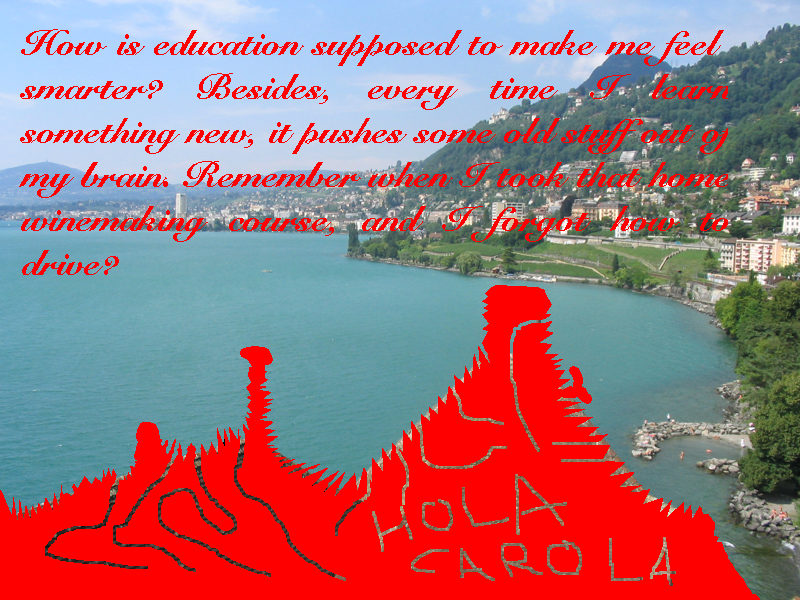
\includegraphics[width=\textwidth]{Goal_image}
%
%    \end{subfigure}
    ~ 
        \begin{subfigure}[b]{0.3\textwidth}
        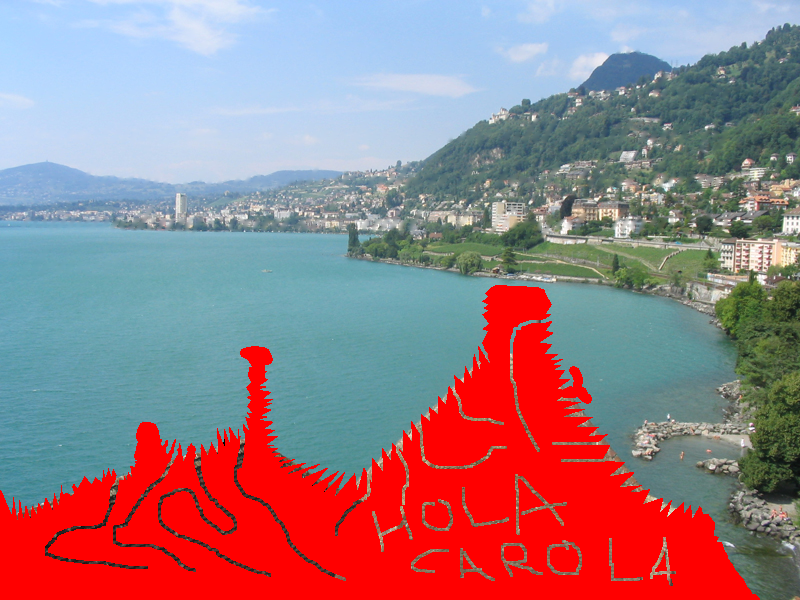
\includegraphics[width=\textwidth]{Goal_inpaint}
	\caption{Inpainting of the red letters in image \ref{img:goal_image}. }
	\label{img:process_01}
    \end{subfigure}
	~
	\begin{subfigure}[b]{0.3\textwidth}
        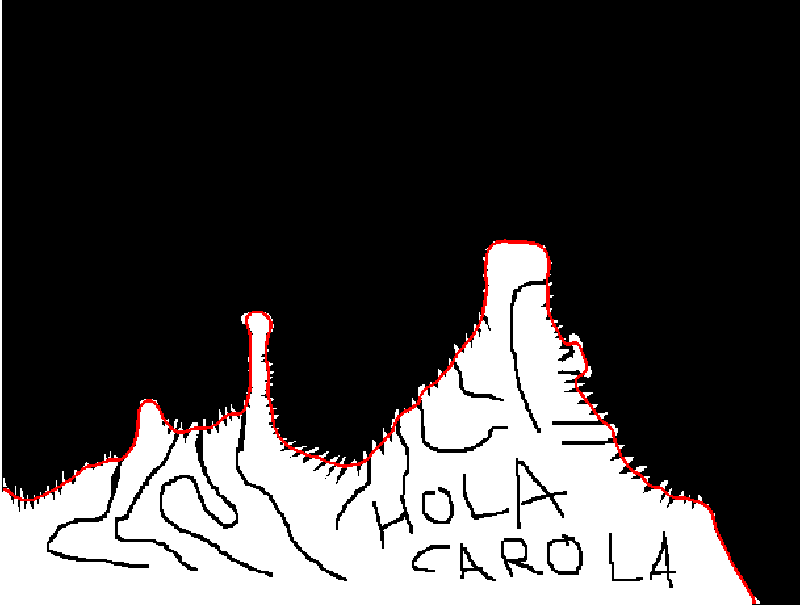
\includegraphics[width=\textwidth]{Goal_segmentation}
	\caption{Segmentation of the red zone remaining in \ref{img:process_01}. }\label{img:process_02}
    \end{subfigure}
    ~ 
        \begin{subfigure}[b]{0.3\textwidth}
        \includegraphics[width=\textwidth]{Goal_completion}
	\caption{One possible final result of the image completion.}
	\label{img:process_03}
    \end{subfigure}
\caption{steps of the algorithm presented on the document. Image \ref{img:process_01} corresponds to section \ref{sec:inpaint}, image \ref{img:process_02} corresponds to section \ref{sec:segmentation} and  image \ref{img:process_03} corresponds to section \ref{sec:completion}.  }
\label{img:process}
\end{figure}



\bibliographystyle{unsrt}
\bibliography{bibliografia}
\end{document}
